%
% Introduction.tex
%
% LulzBot Mini Developer's Guide
%
% Copyright (C) 2014 Aleph Objects, Inc.
%
% This document is licensed under the Creative Commons Attribution 4.0
% International Public License (CC BY-SA 4.0) by Aleph Objects, Inc.
%

\section{LulzBot Mini}
The LulzBot Mini is a 3D Printer currently under development. The
abbreviated name is mini-dev.

The source files are available here:

\href{http://devel.lulzbot.com/mini/}{http://devel.lulzbot.com/mini/}

\section{Versions}
Each new version of the mini-dev has a new name, with the next letter in the alphabet.

\begin{itemize}
  \item Azalea - First Prototype
  \item Begonia - Second Prototype, being built now
  \item Camellia - Third Prototype
  \item Daffodil - First Production batch
\end{itemize}

\section{Begonia Photos}

\begin{figure}[H]
\centering
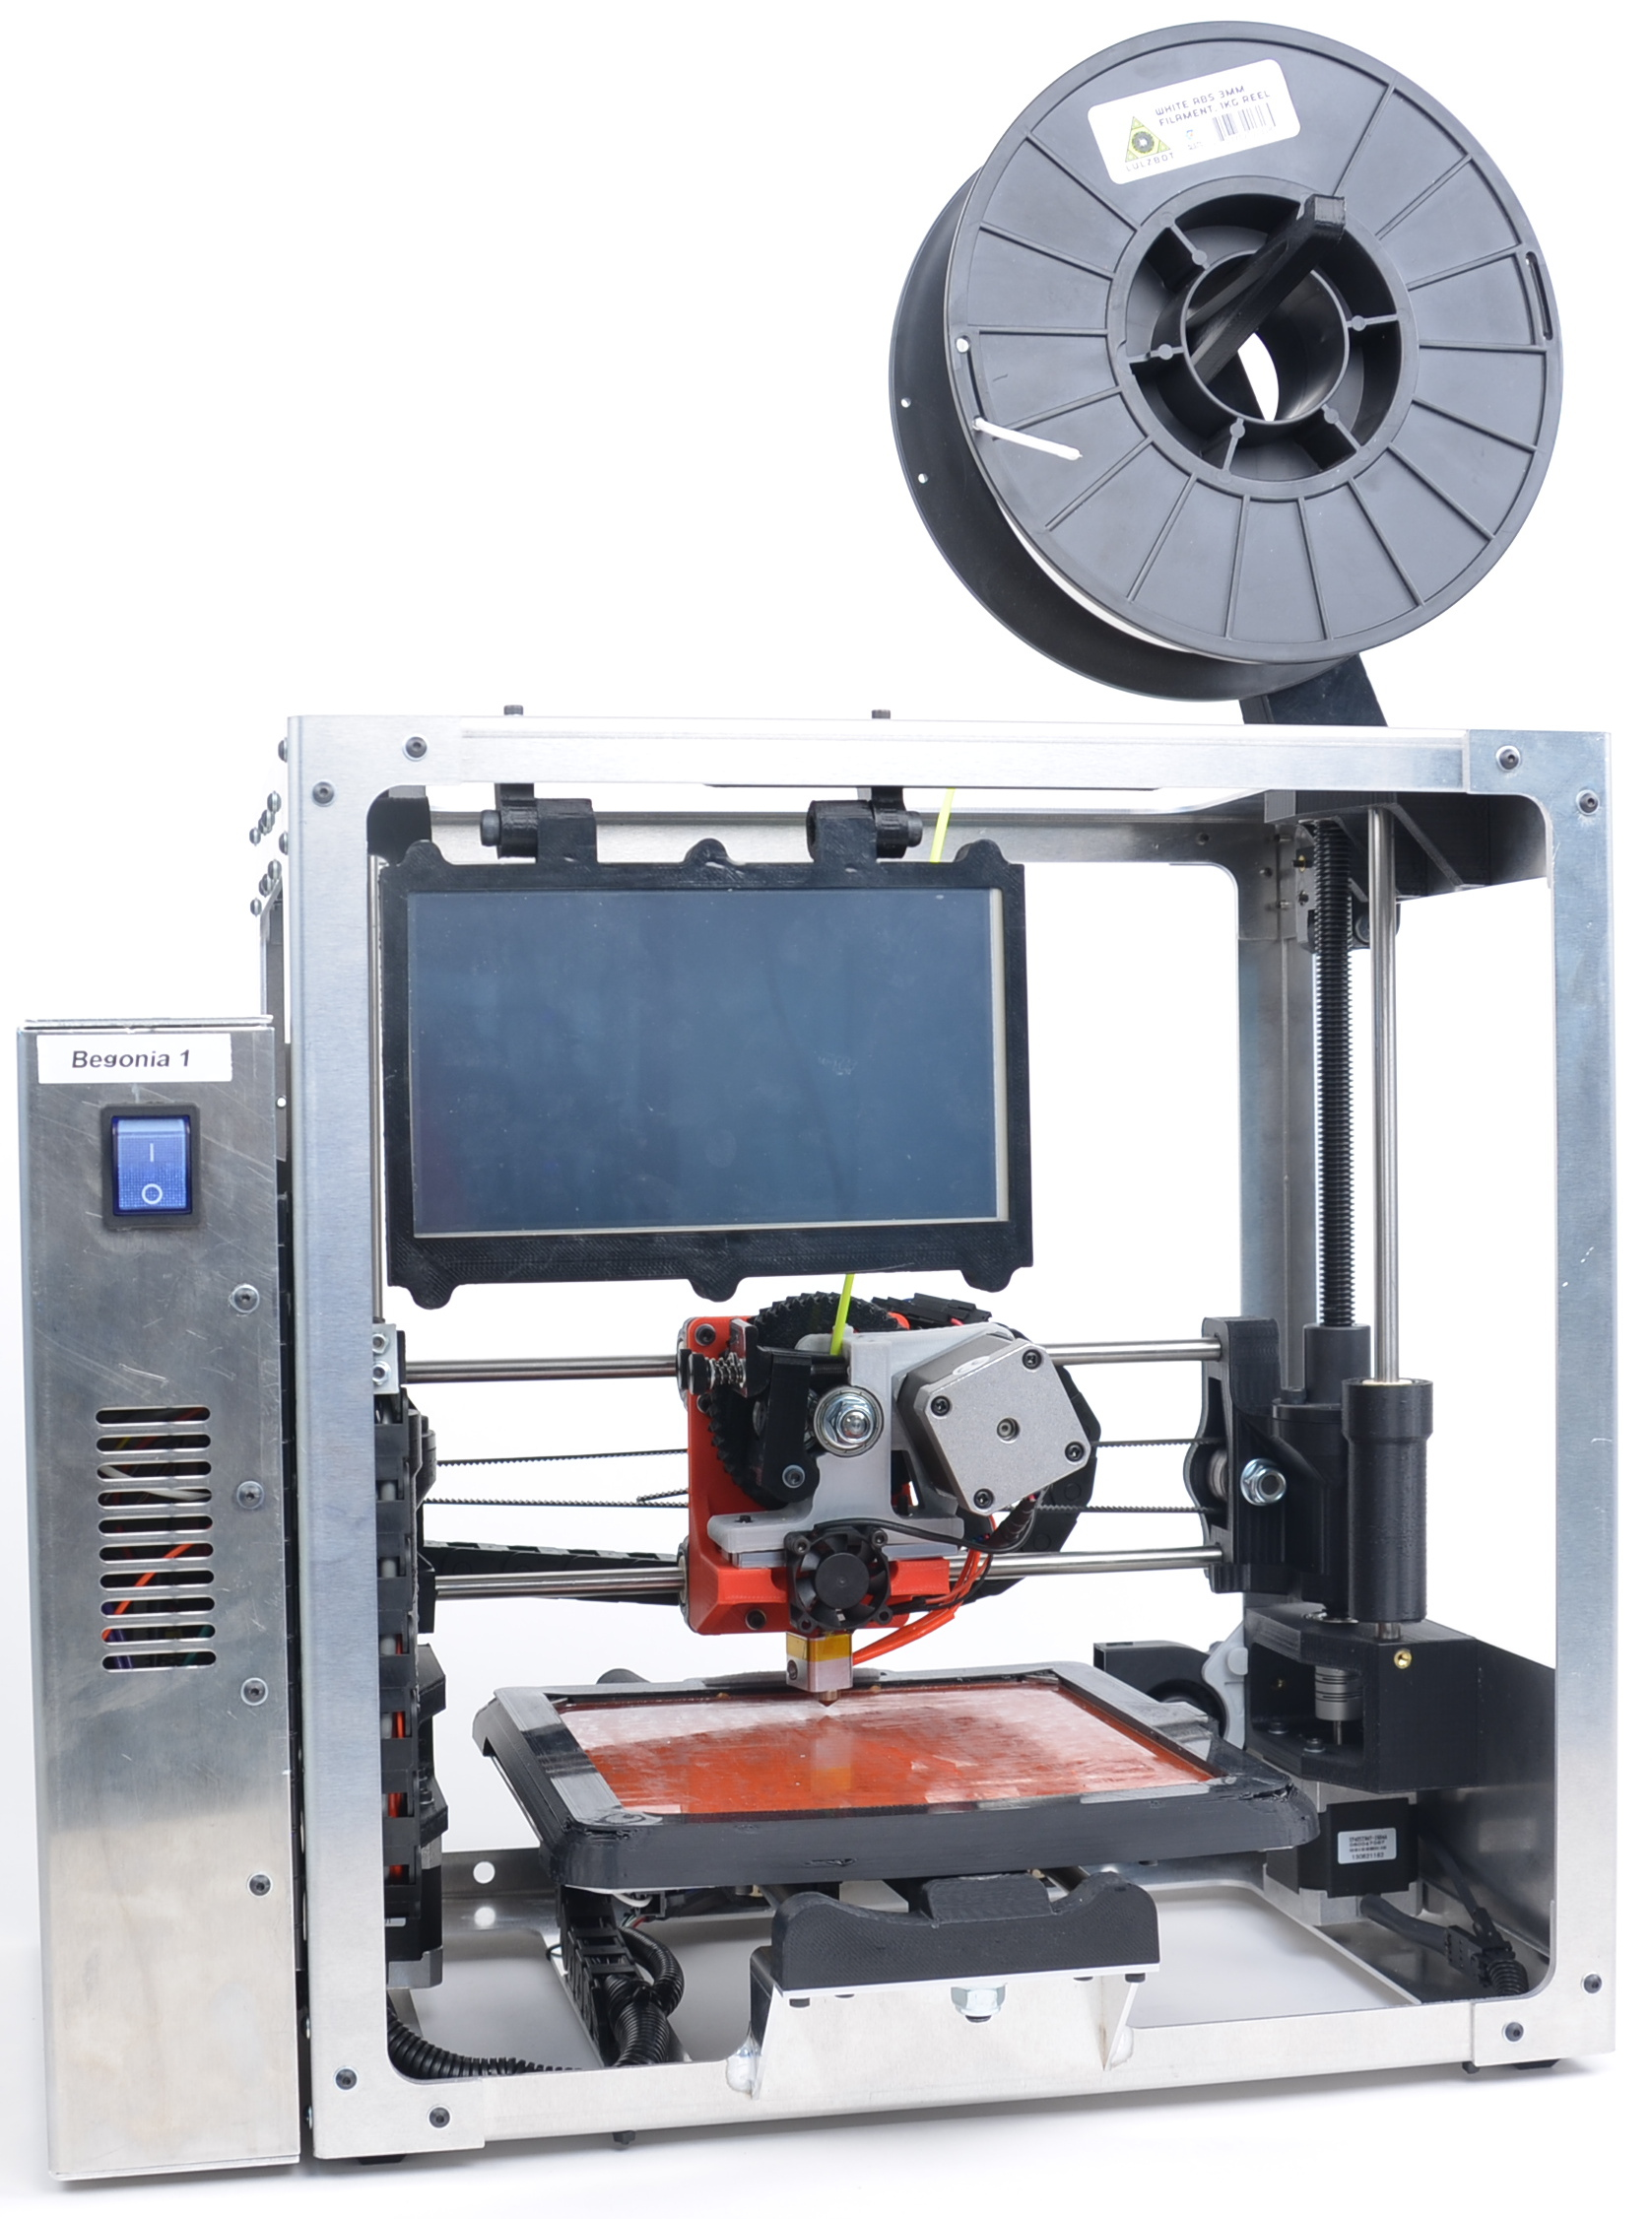
\includegraphics[keepaspectratio=true,angle=0,height=1.0\textheight,width=1.0\textwidth]{begonia/begonia-front.jpg}
\caption{Begonia Front Photo}
\label{fig:begfrontfoto}
\end{figure}

\begin{figure}[H]
\centering
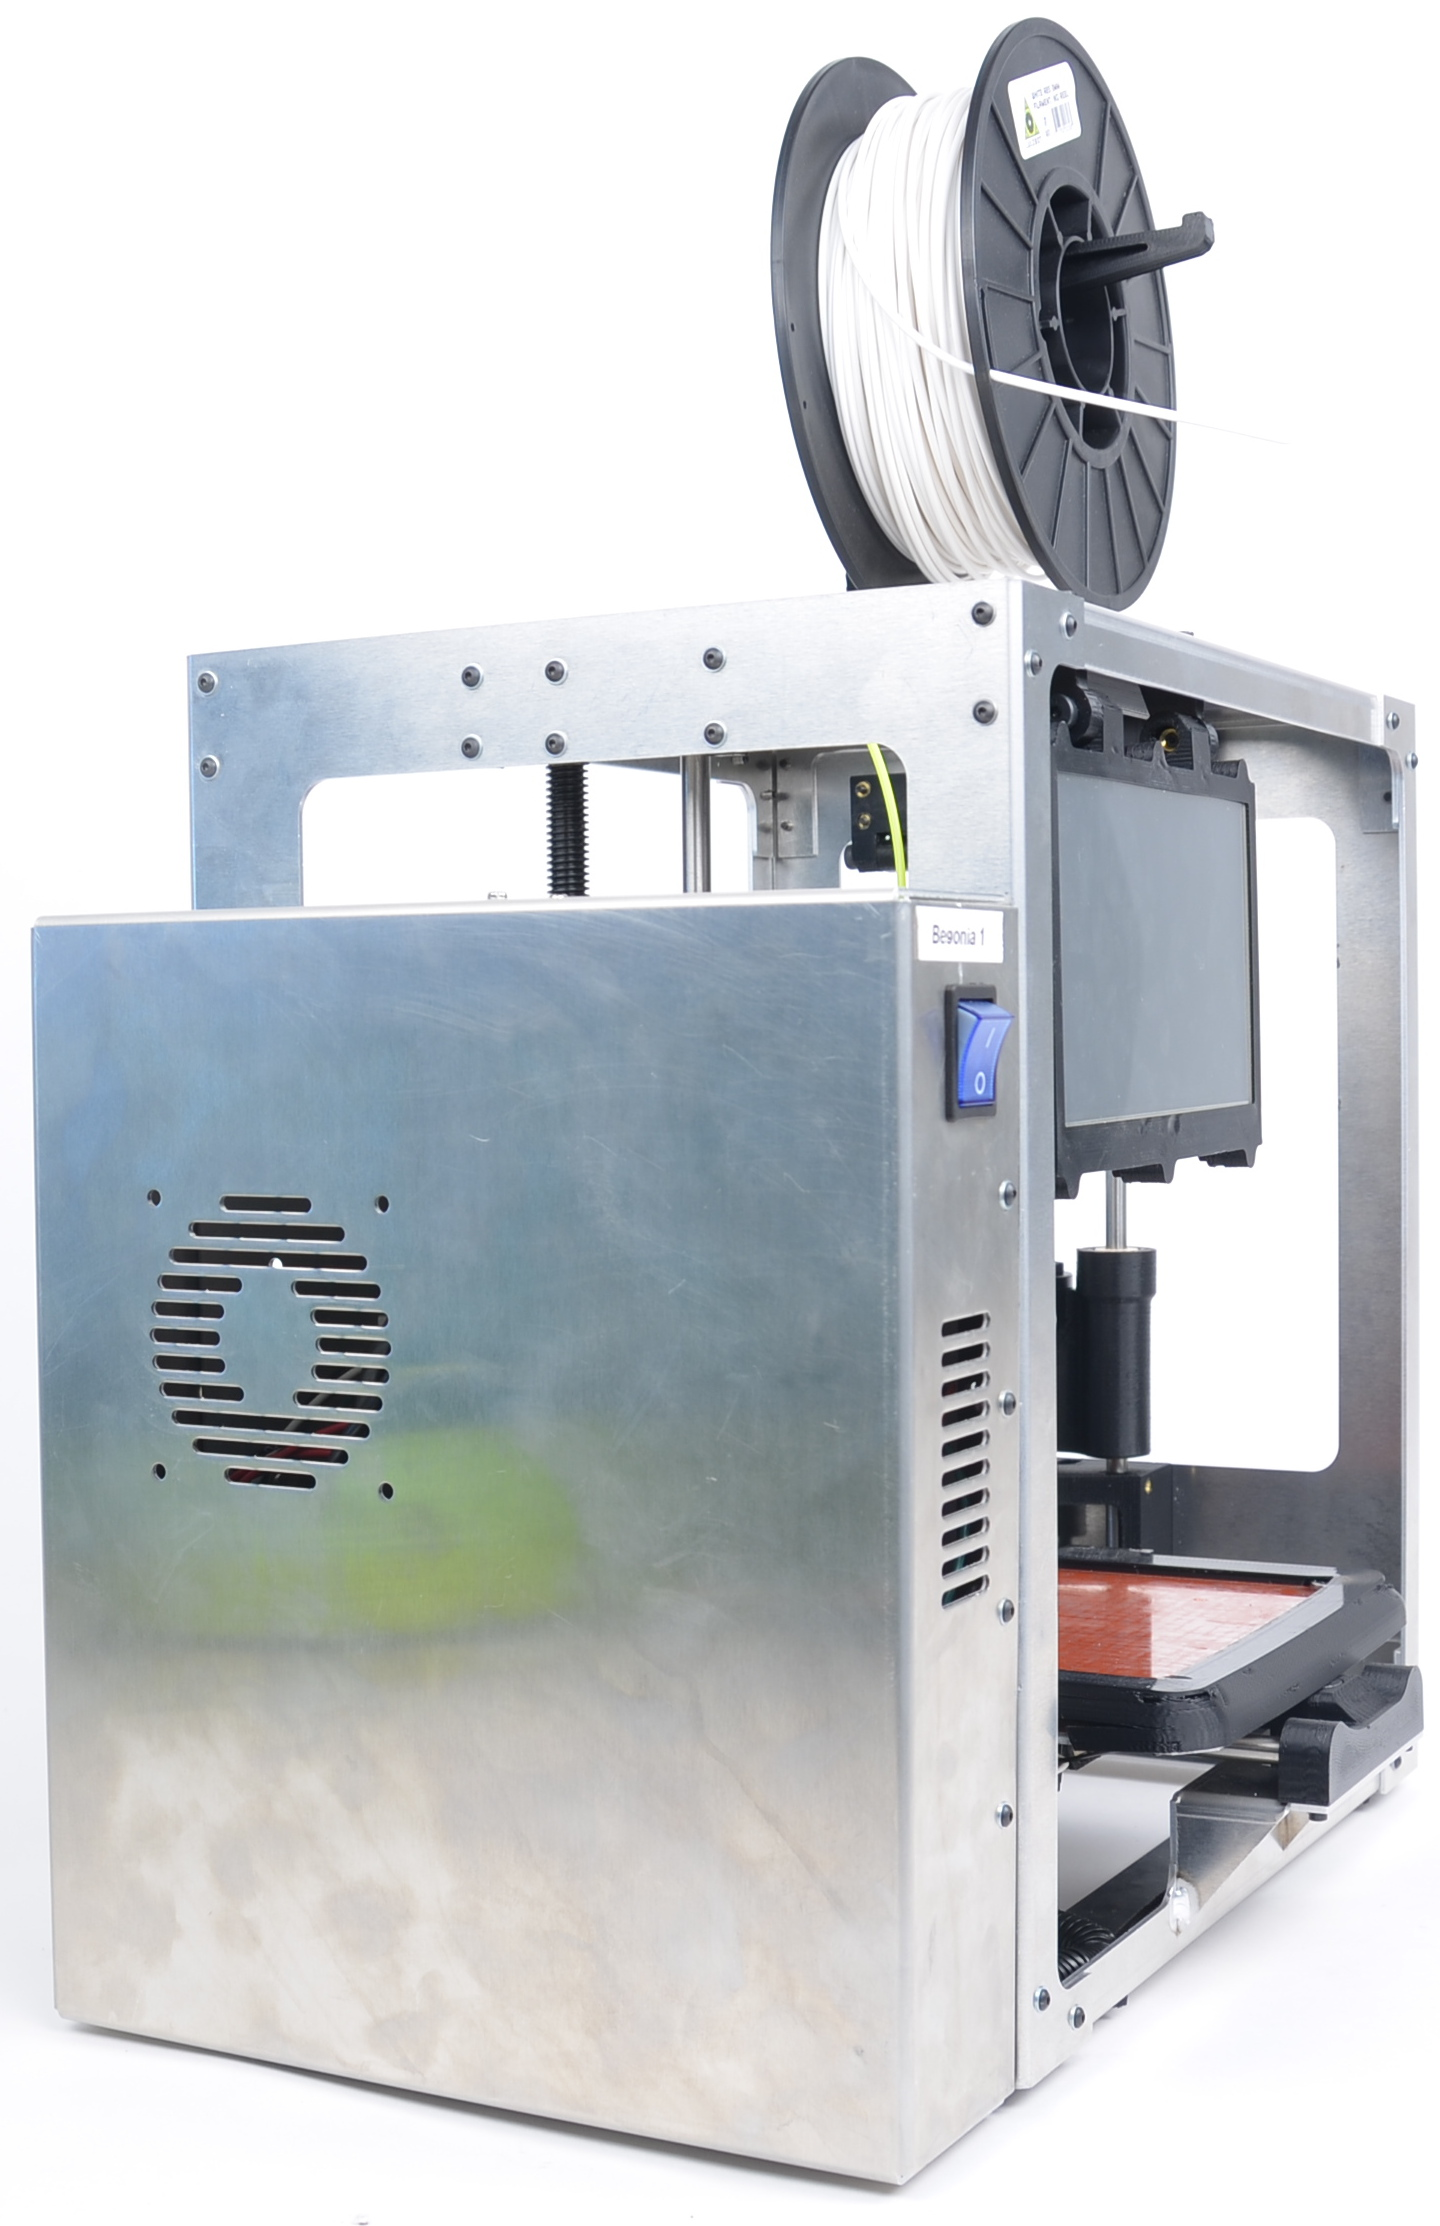
\includegraphics[keepaspectratio=true,angle=0,height=1.0\textheight,width=1.0\textwidth]{begonia/begonia-left.jpg}
\caption{Begonia Left Photo}
\label{fig:begleftfoto}
\end{figure}

\begin{figure}[H]
\centering
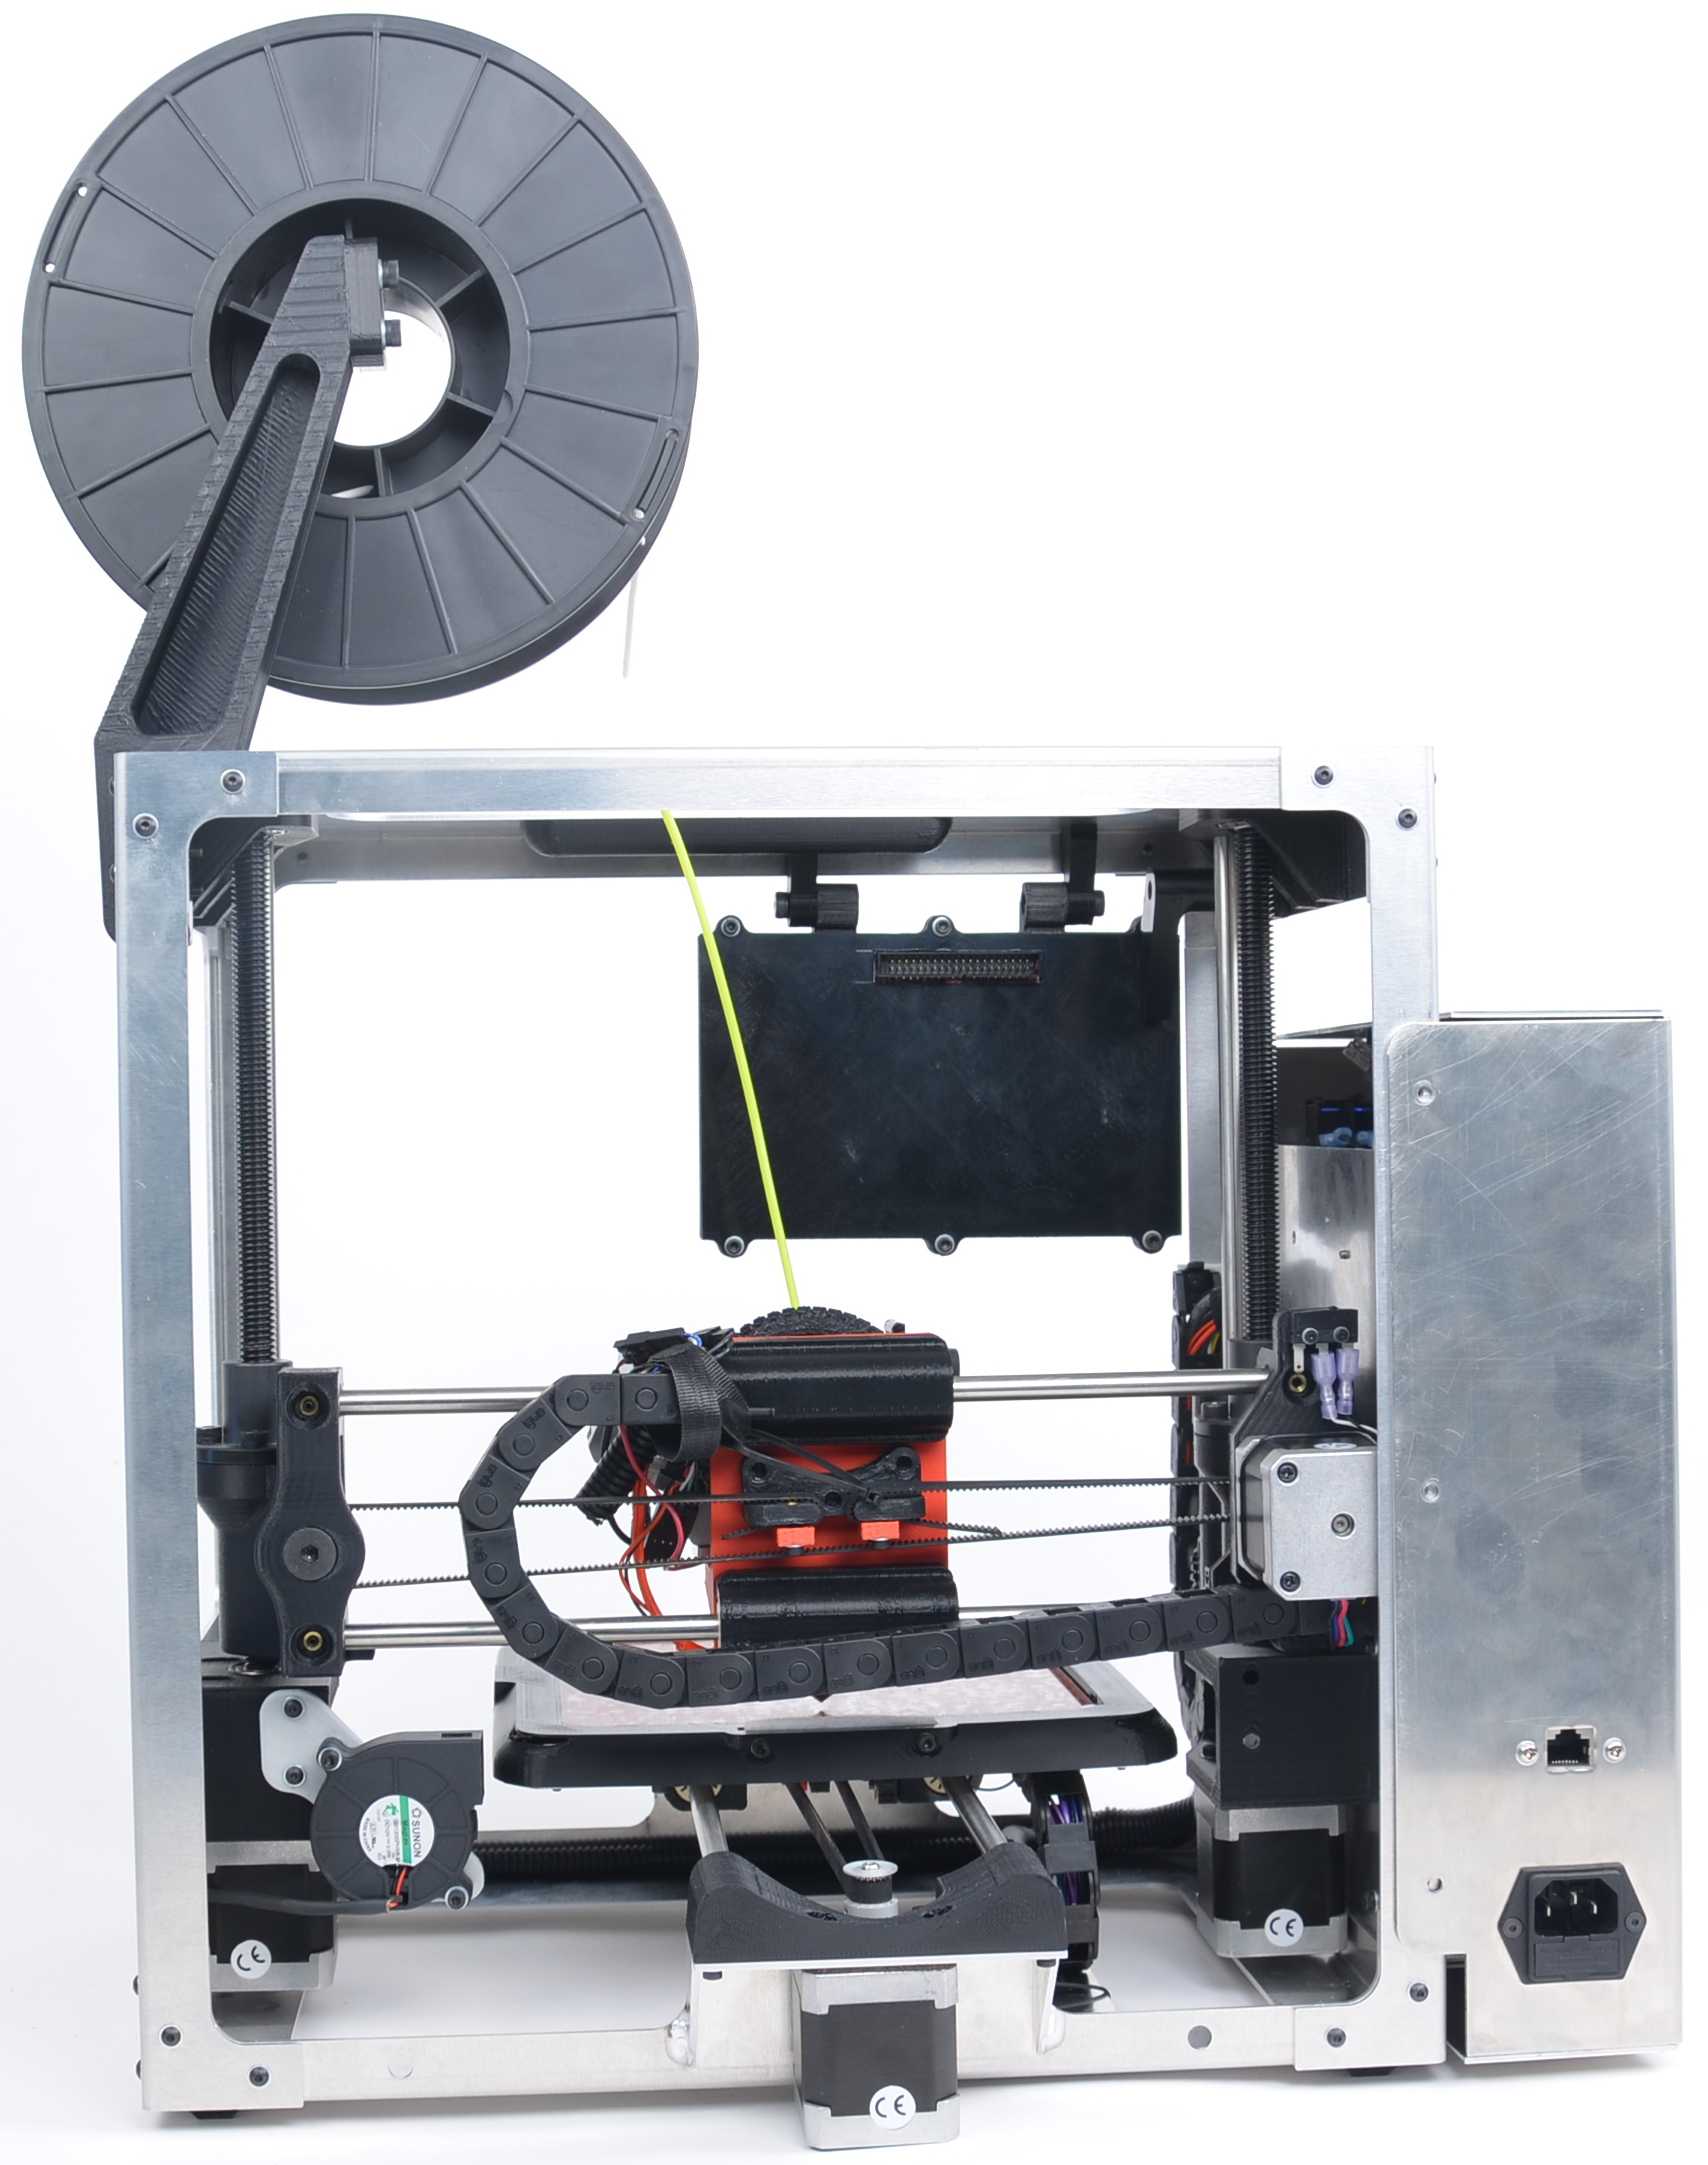
\includegraphics[keepaspectratio=true,angle=0,height=1.0\textheight,width=1.0\textwidth]{begonia/begonia-back.jpg}
\caption{Begonia Back Photo}
\label{fig:begbackfoto}
\end{figure}

\begin{figure}[H]
\centering
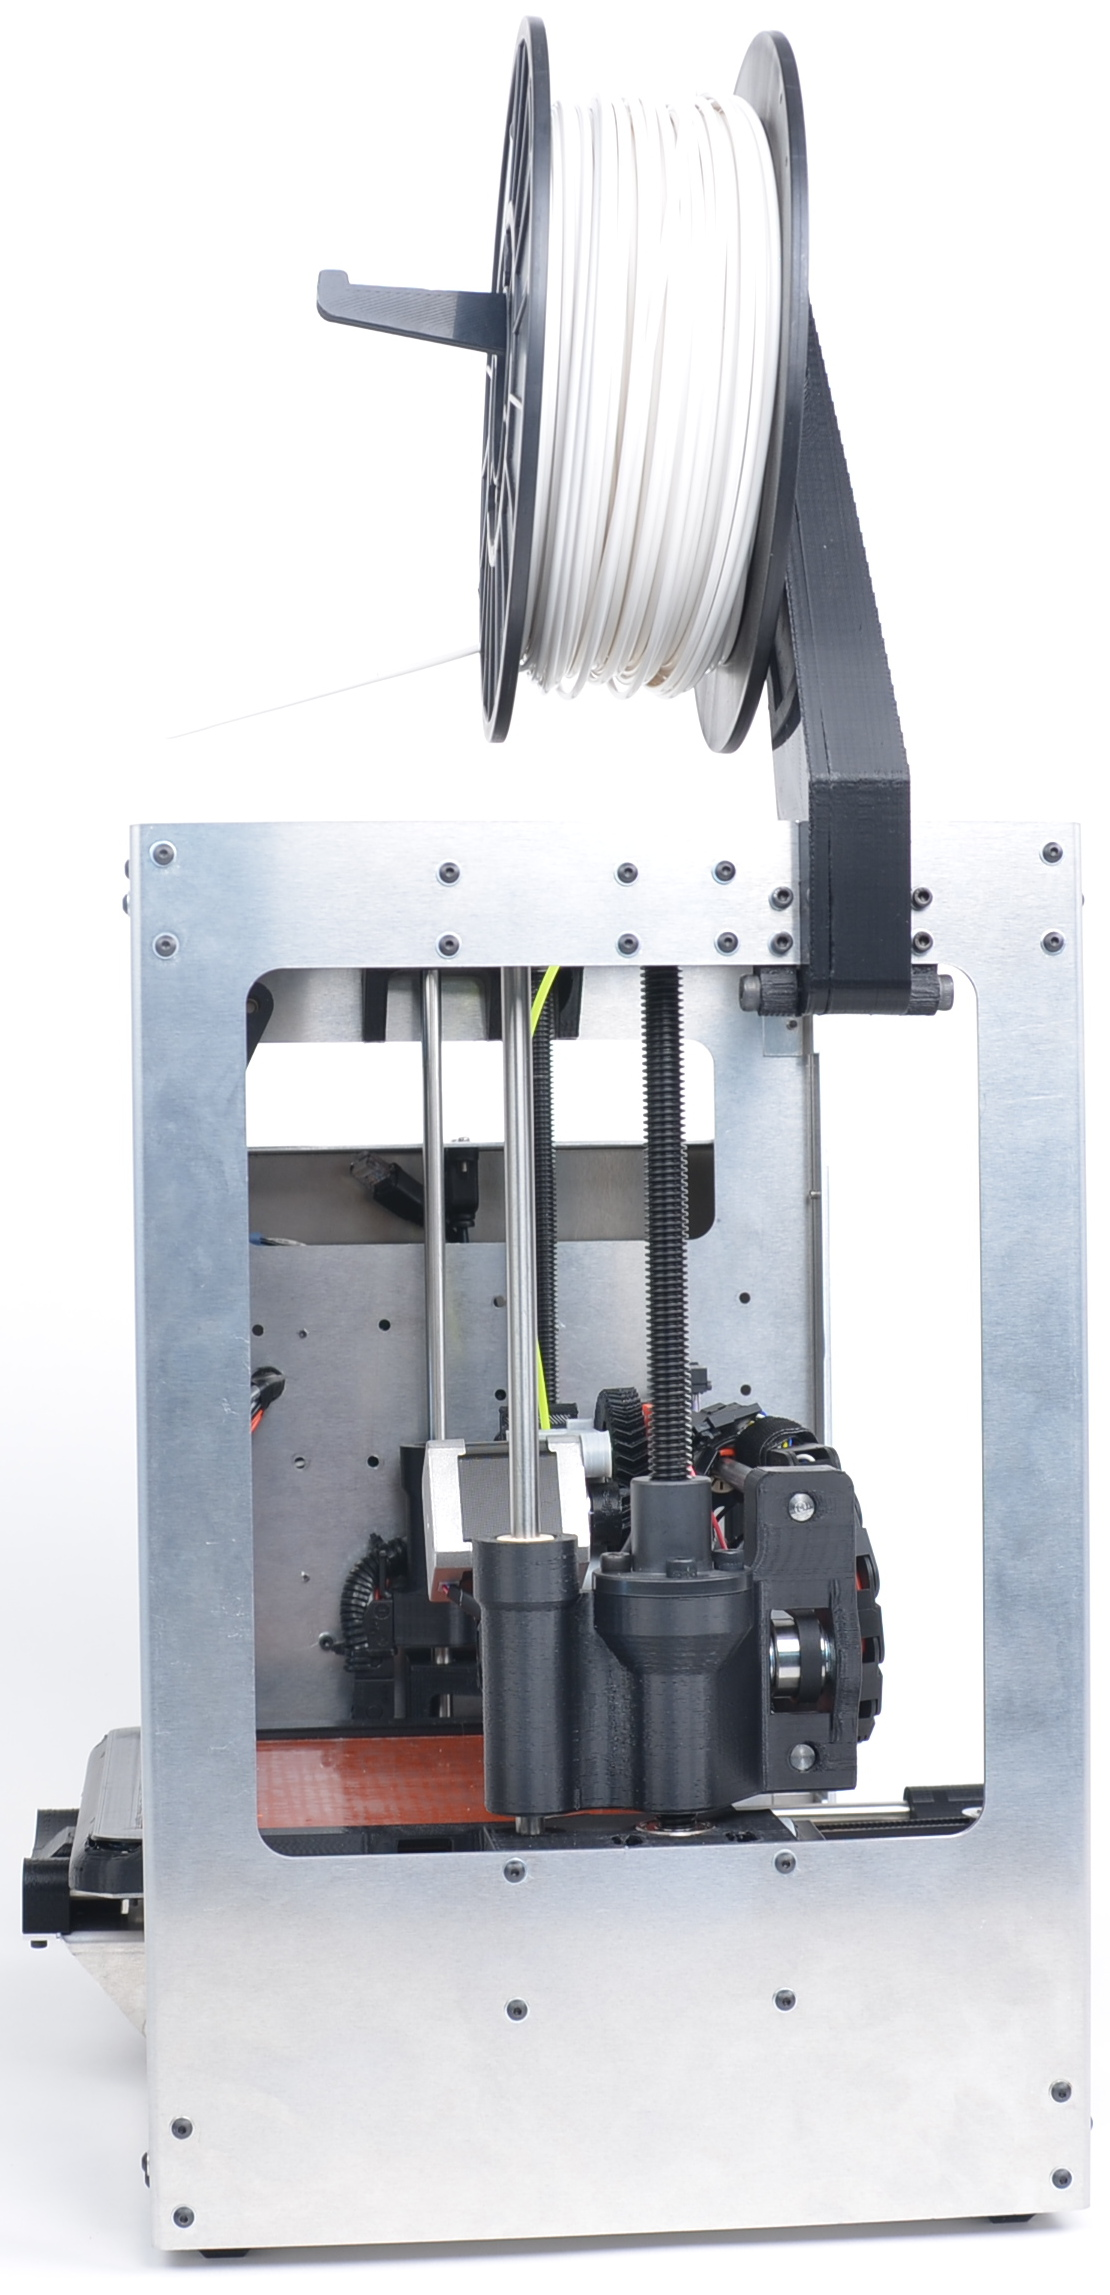
\includegraphics[keepaspectratio=true,angle=0,height=1.0\textheight,width=1.0\textwidth]{begonia/begonia-right.jpg}
\caption{Begonia Right Photo}
\label{fig:begrightfoto}
\end{figure}

\begin{figure}[H]
\centering
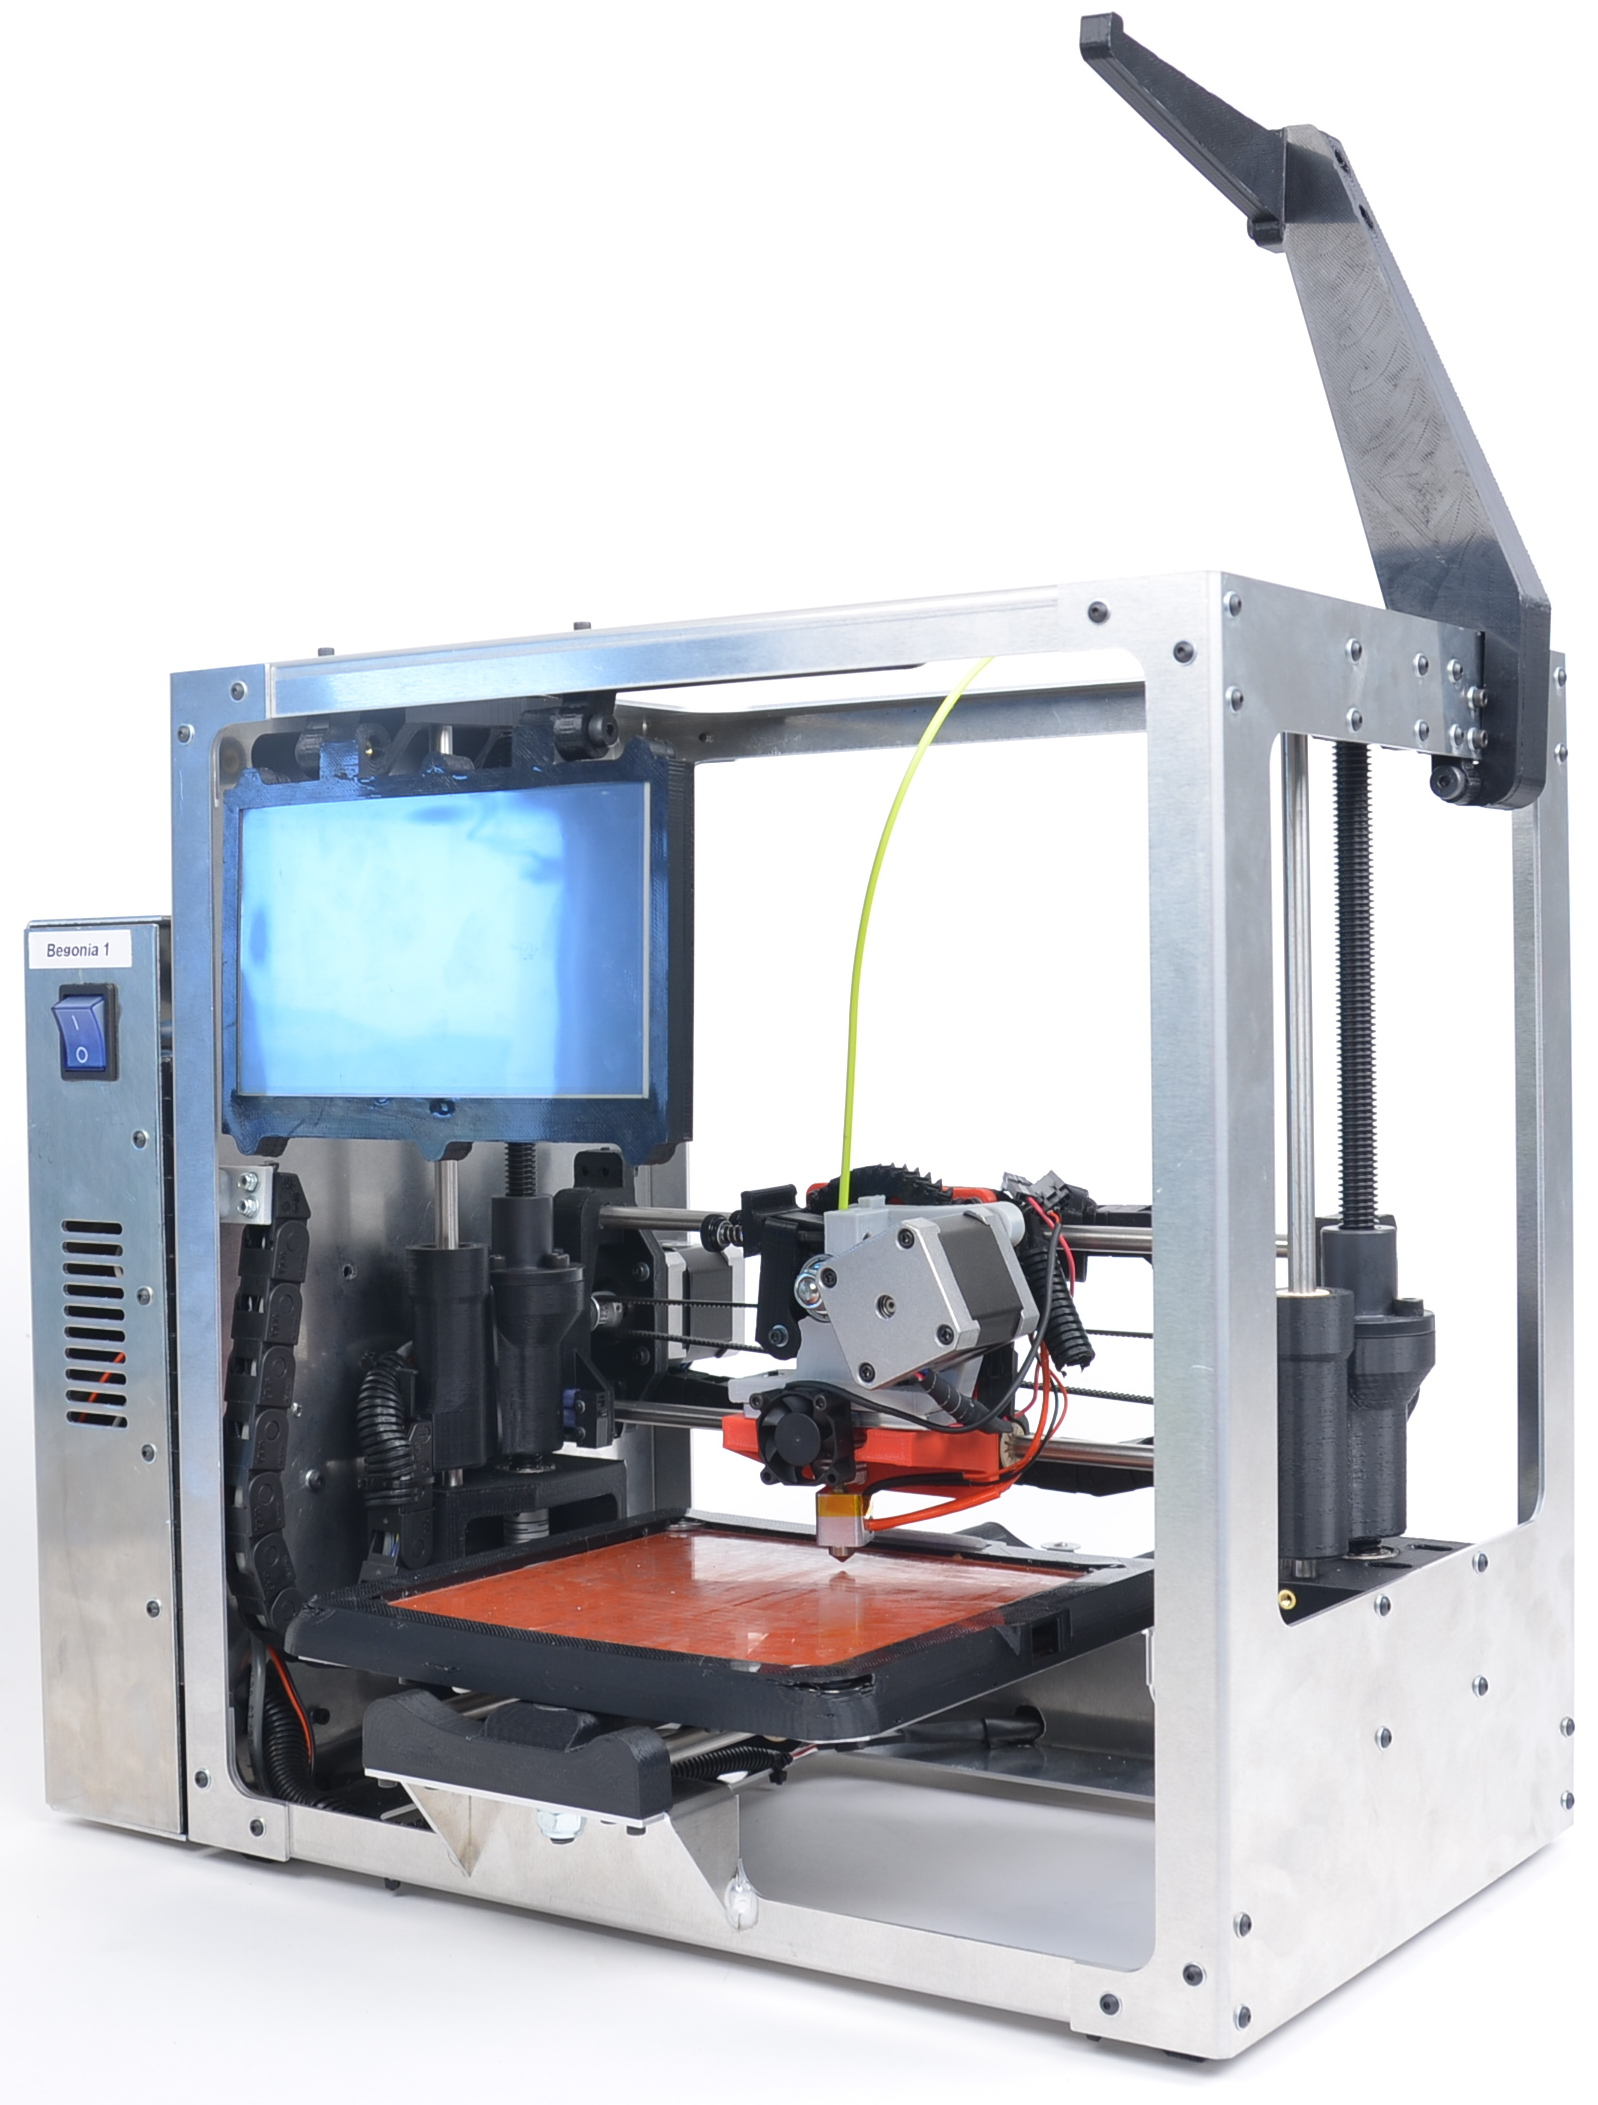
\includegraphics[keepaspectratio=true,angle=0,height=1.0\textheight,width=1.0\textwidth]{begonia/begonia-armup.jpg}
\caption{Begonia Spool Arm Up Photo}
\label{fig:begarmup}
\end{figure}

\begin{figure}[H]
\centering
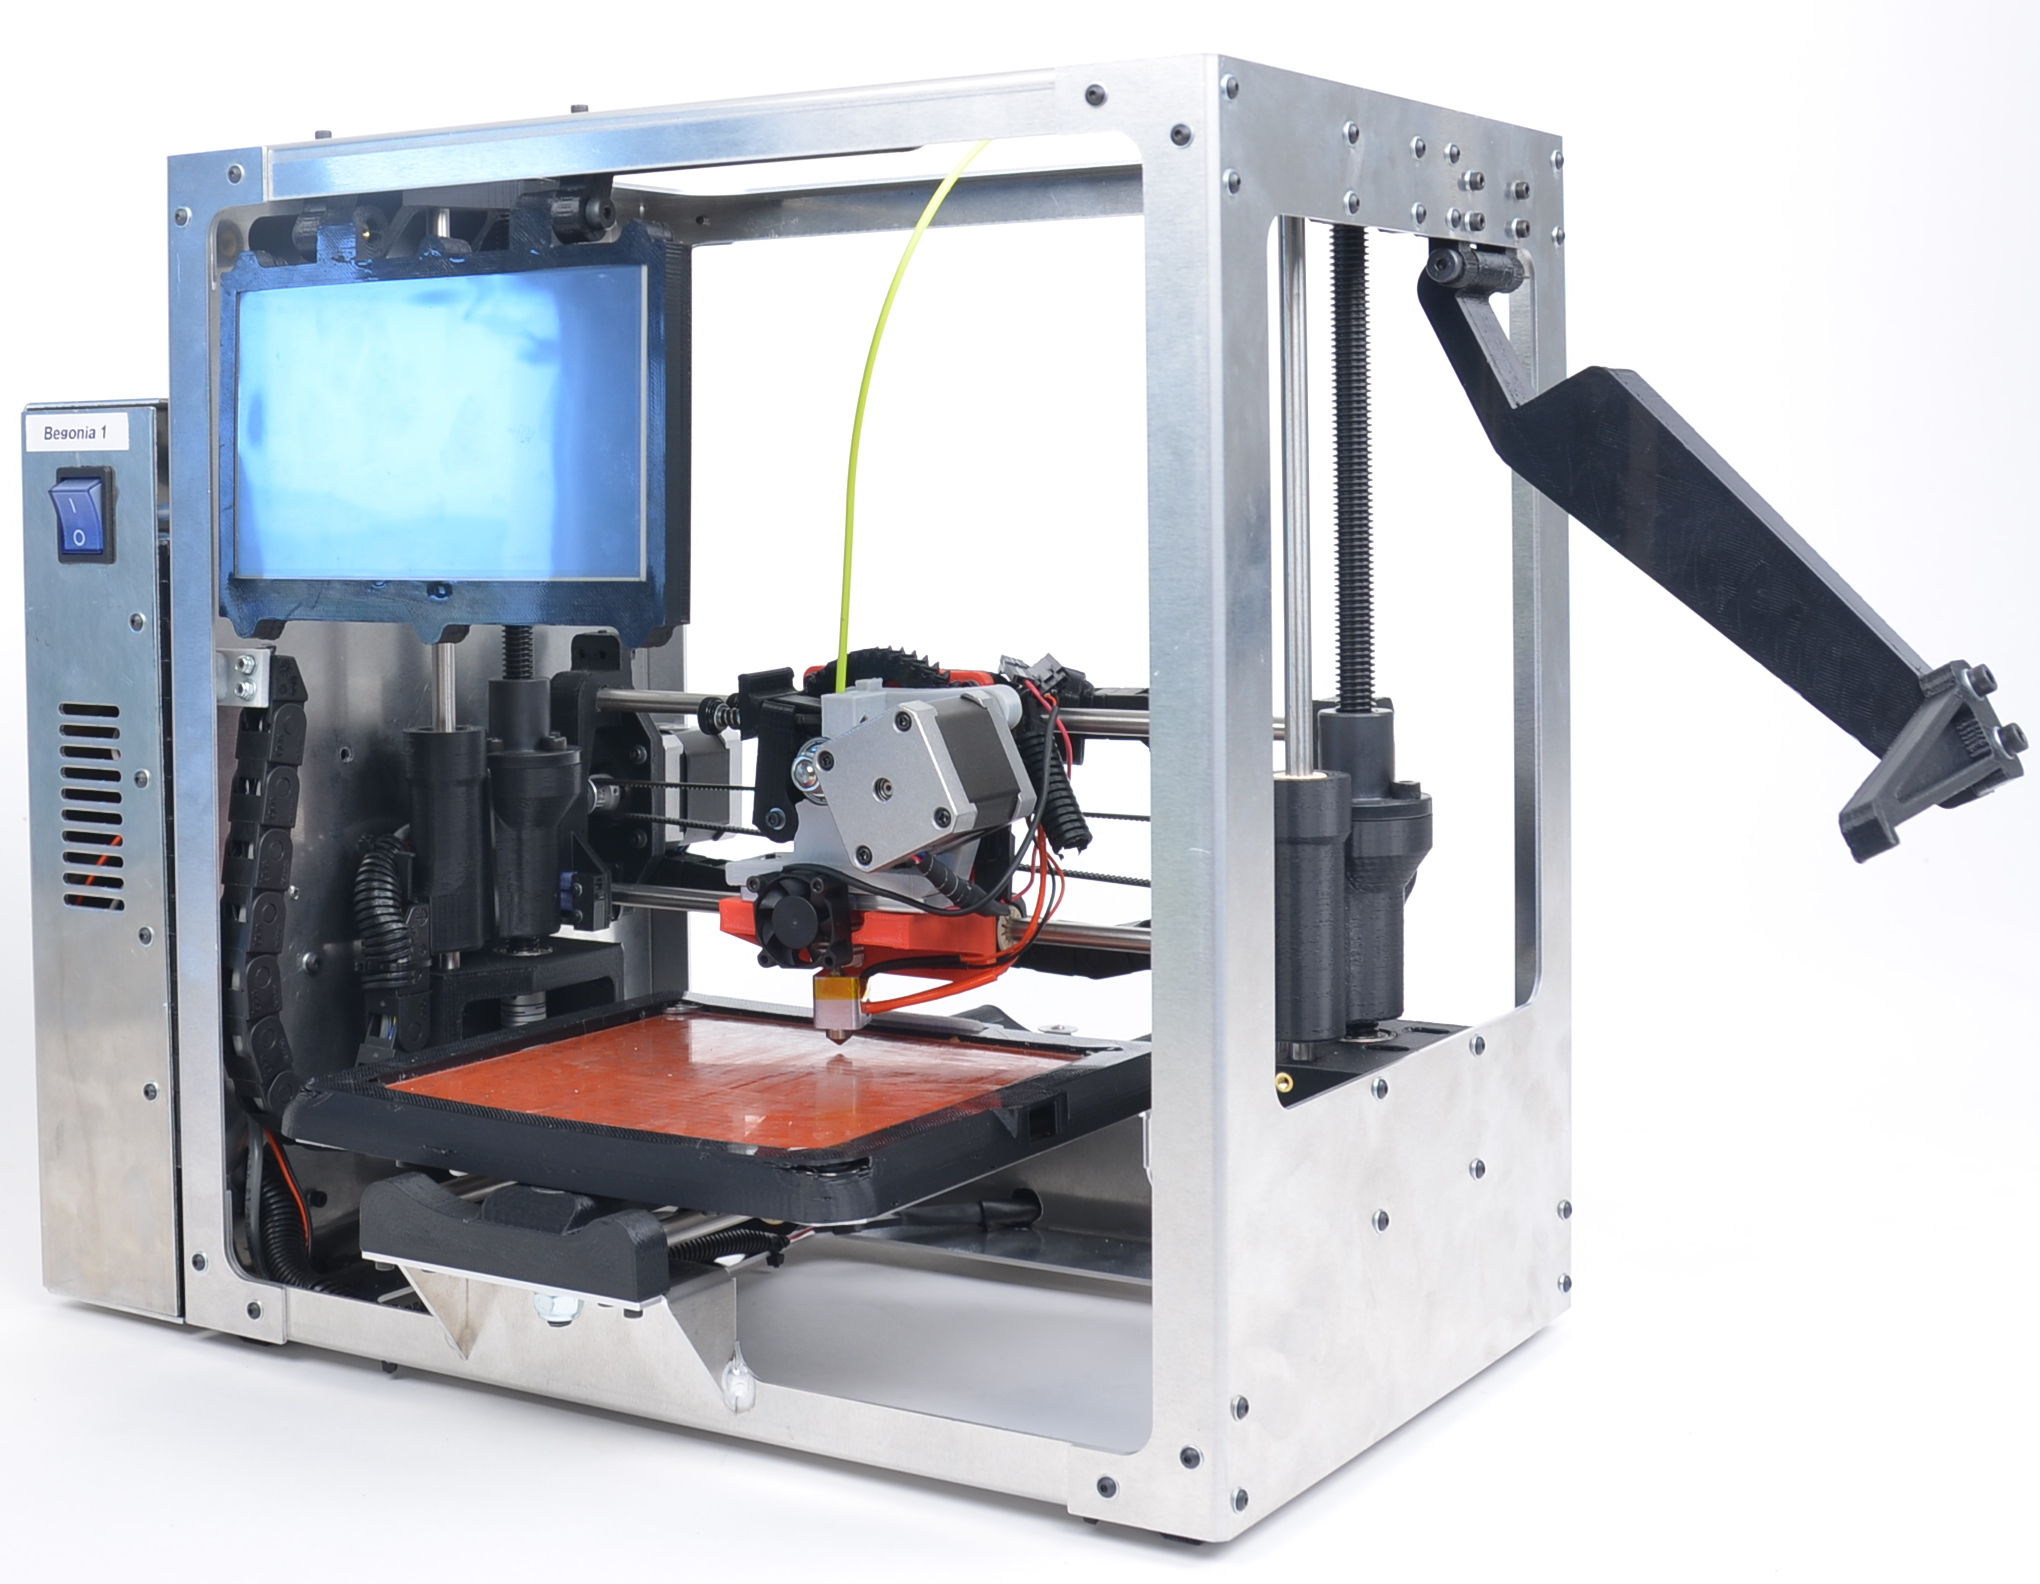
\includegraphics[keepaspectratio=true,angle=0,height=1.0\textheight,width=1.0\textwidth]{begonia/begonia-armdown.jpg}
\caption{Begonia Spool Arm Down Photo}
\label{fig:begarmdown}
\end{figure}

\begin{figure}[H]
\centering
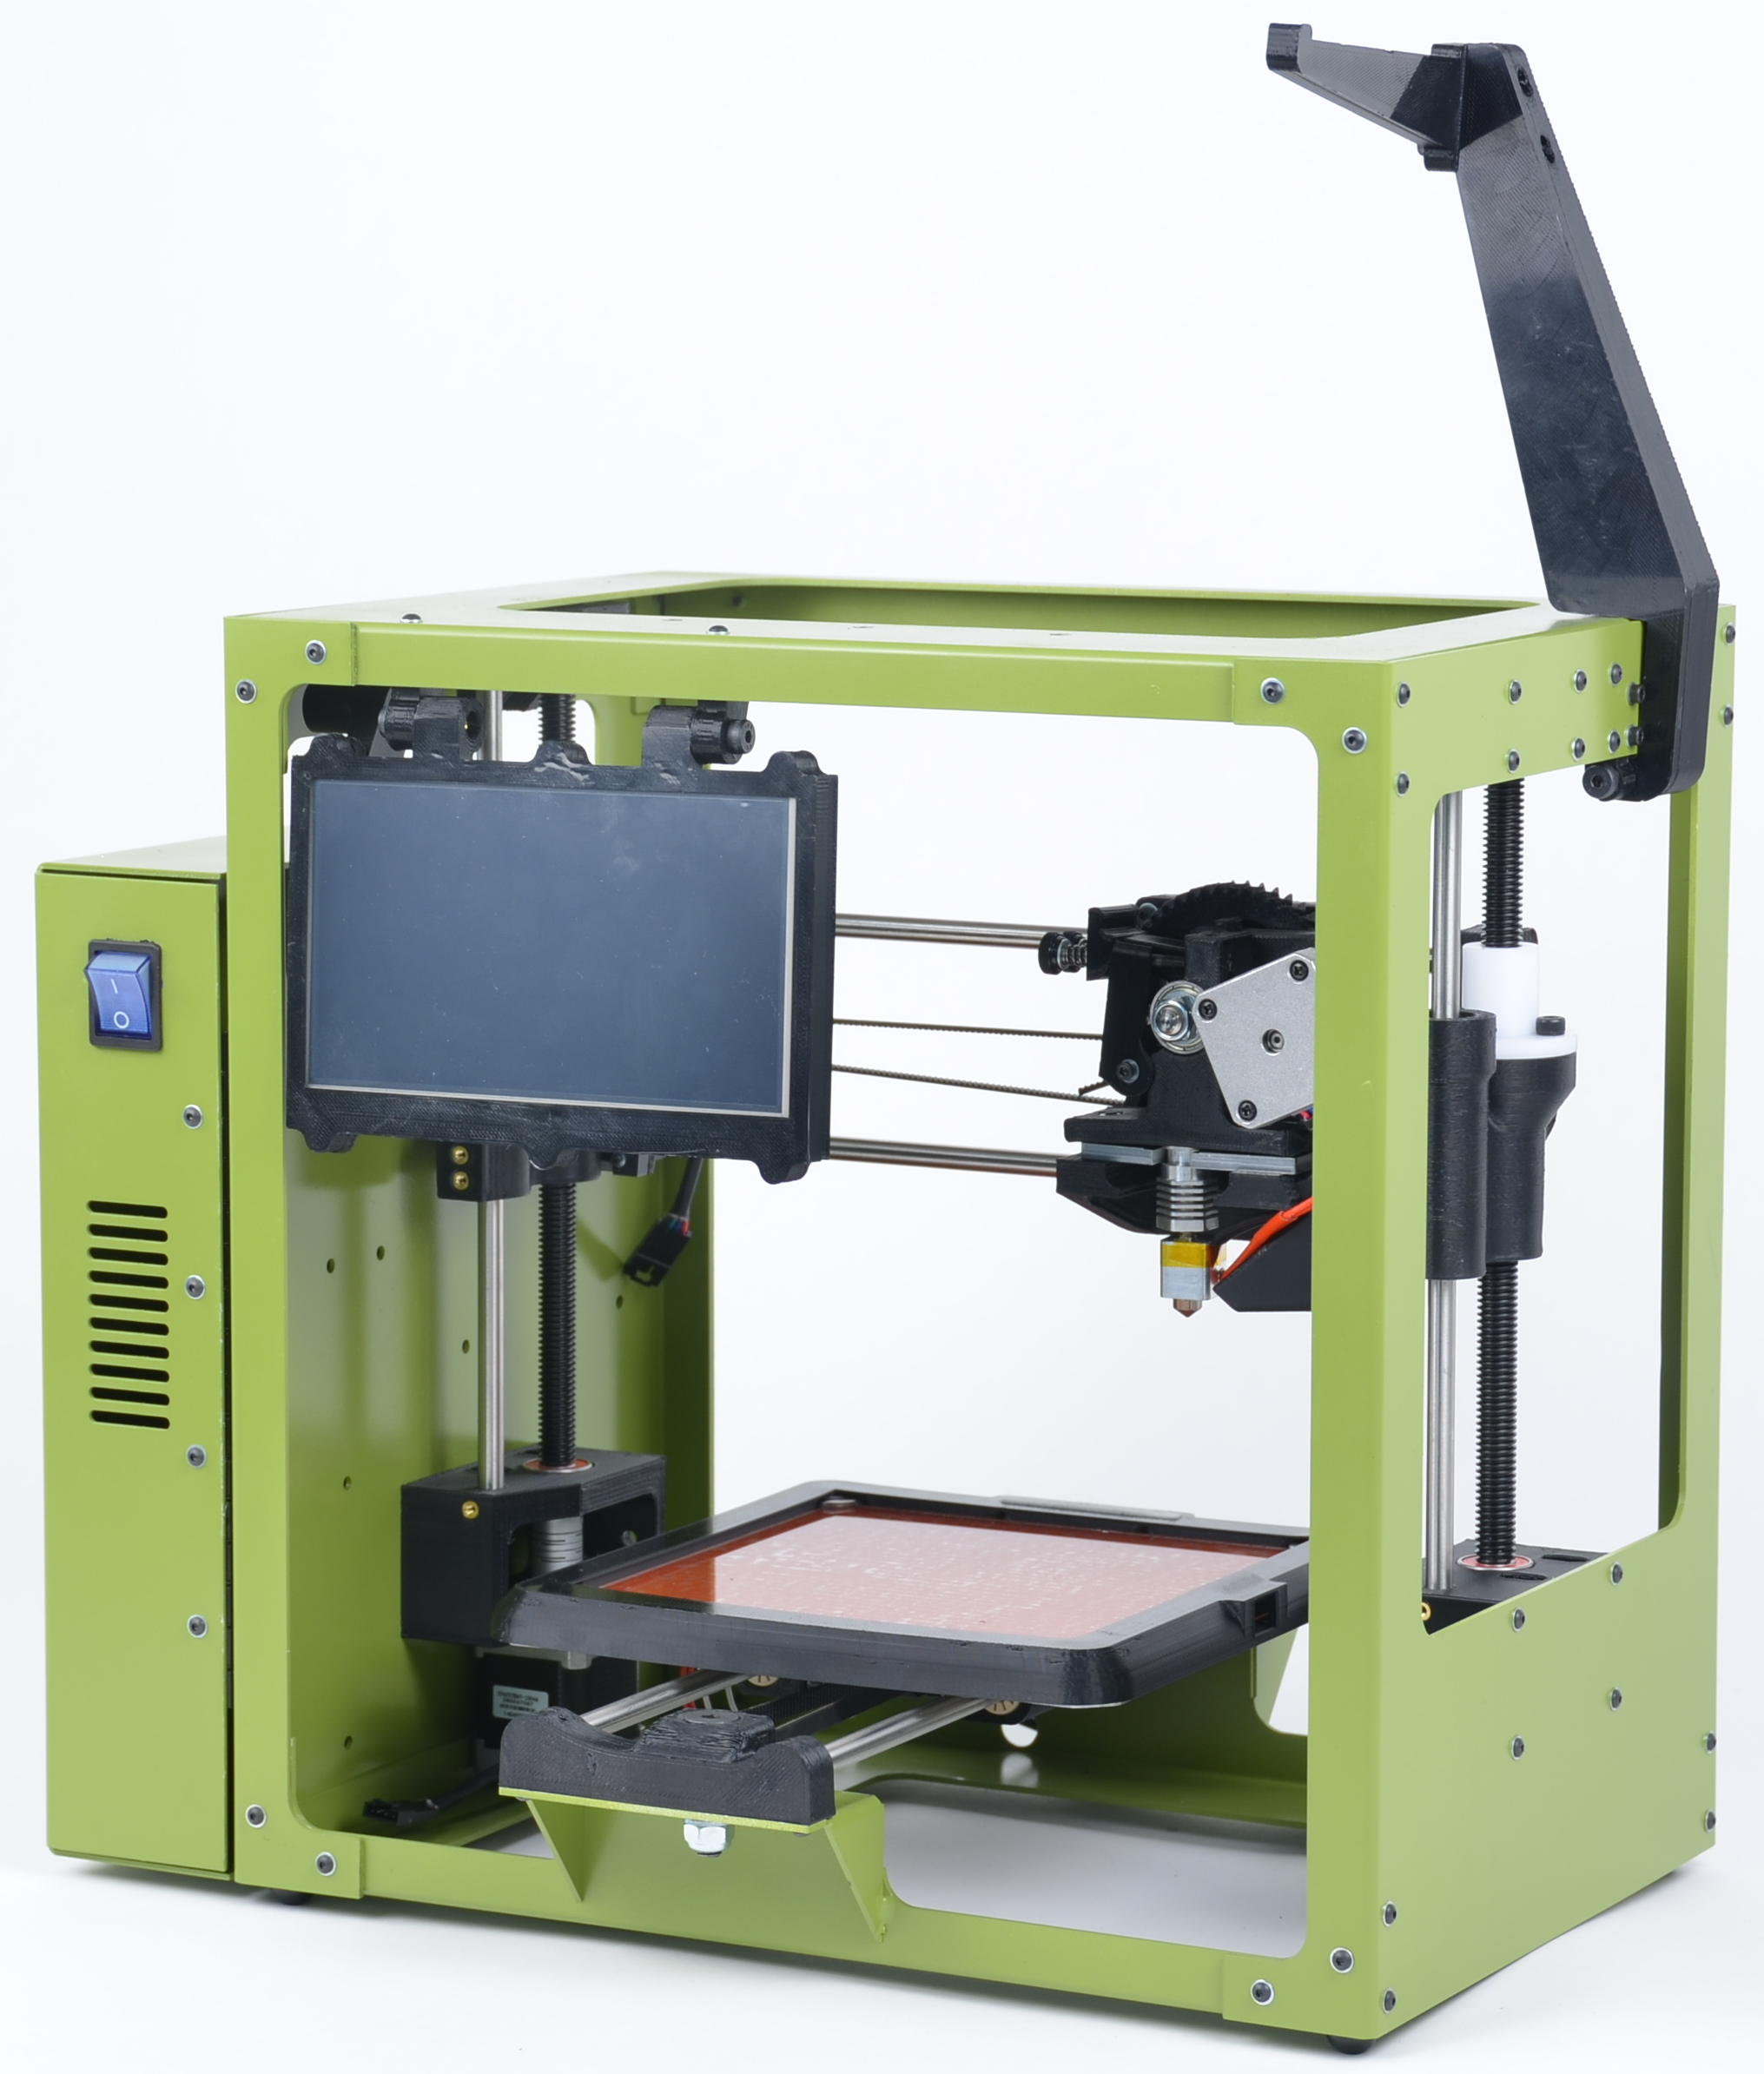
\includegraphics[keepaspectratio=true,angle=0,height=1.0\textheight,width=1.0\textwidth]{begonia/begonia-green.jpg}
\caption{Begonia Green Color Scheme Photo}
\label{fig:beggreen}
\end{figure}

\begin{figure}[H]
\centering
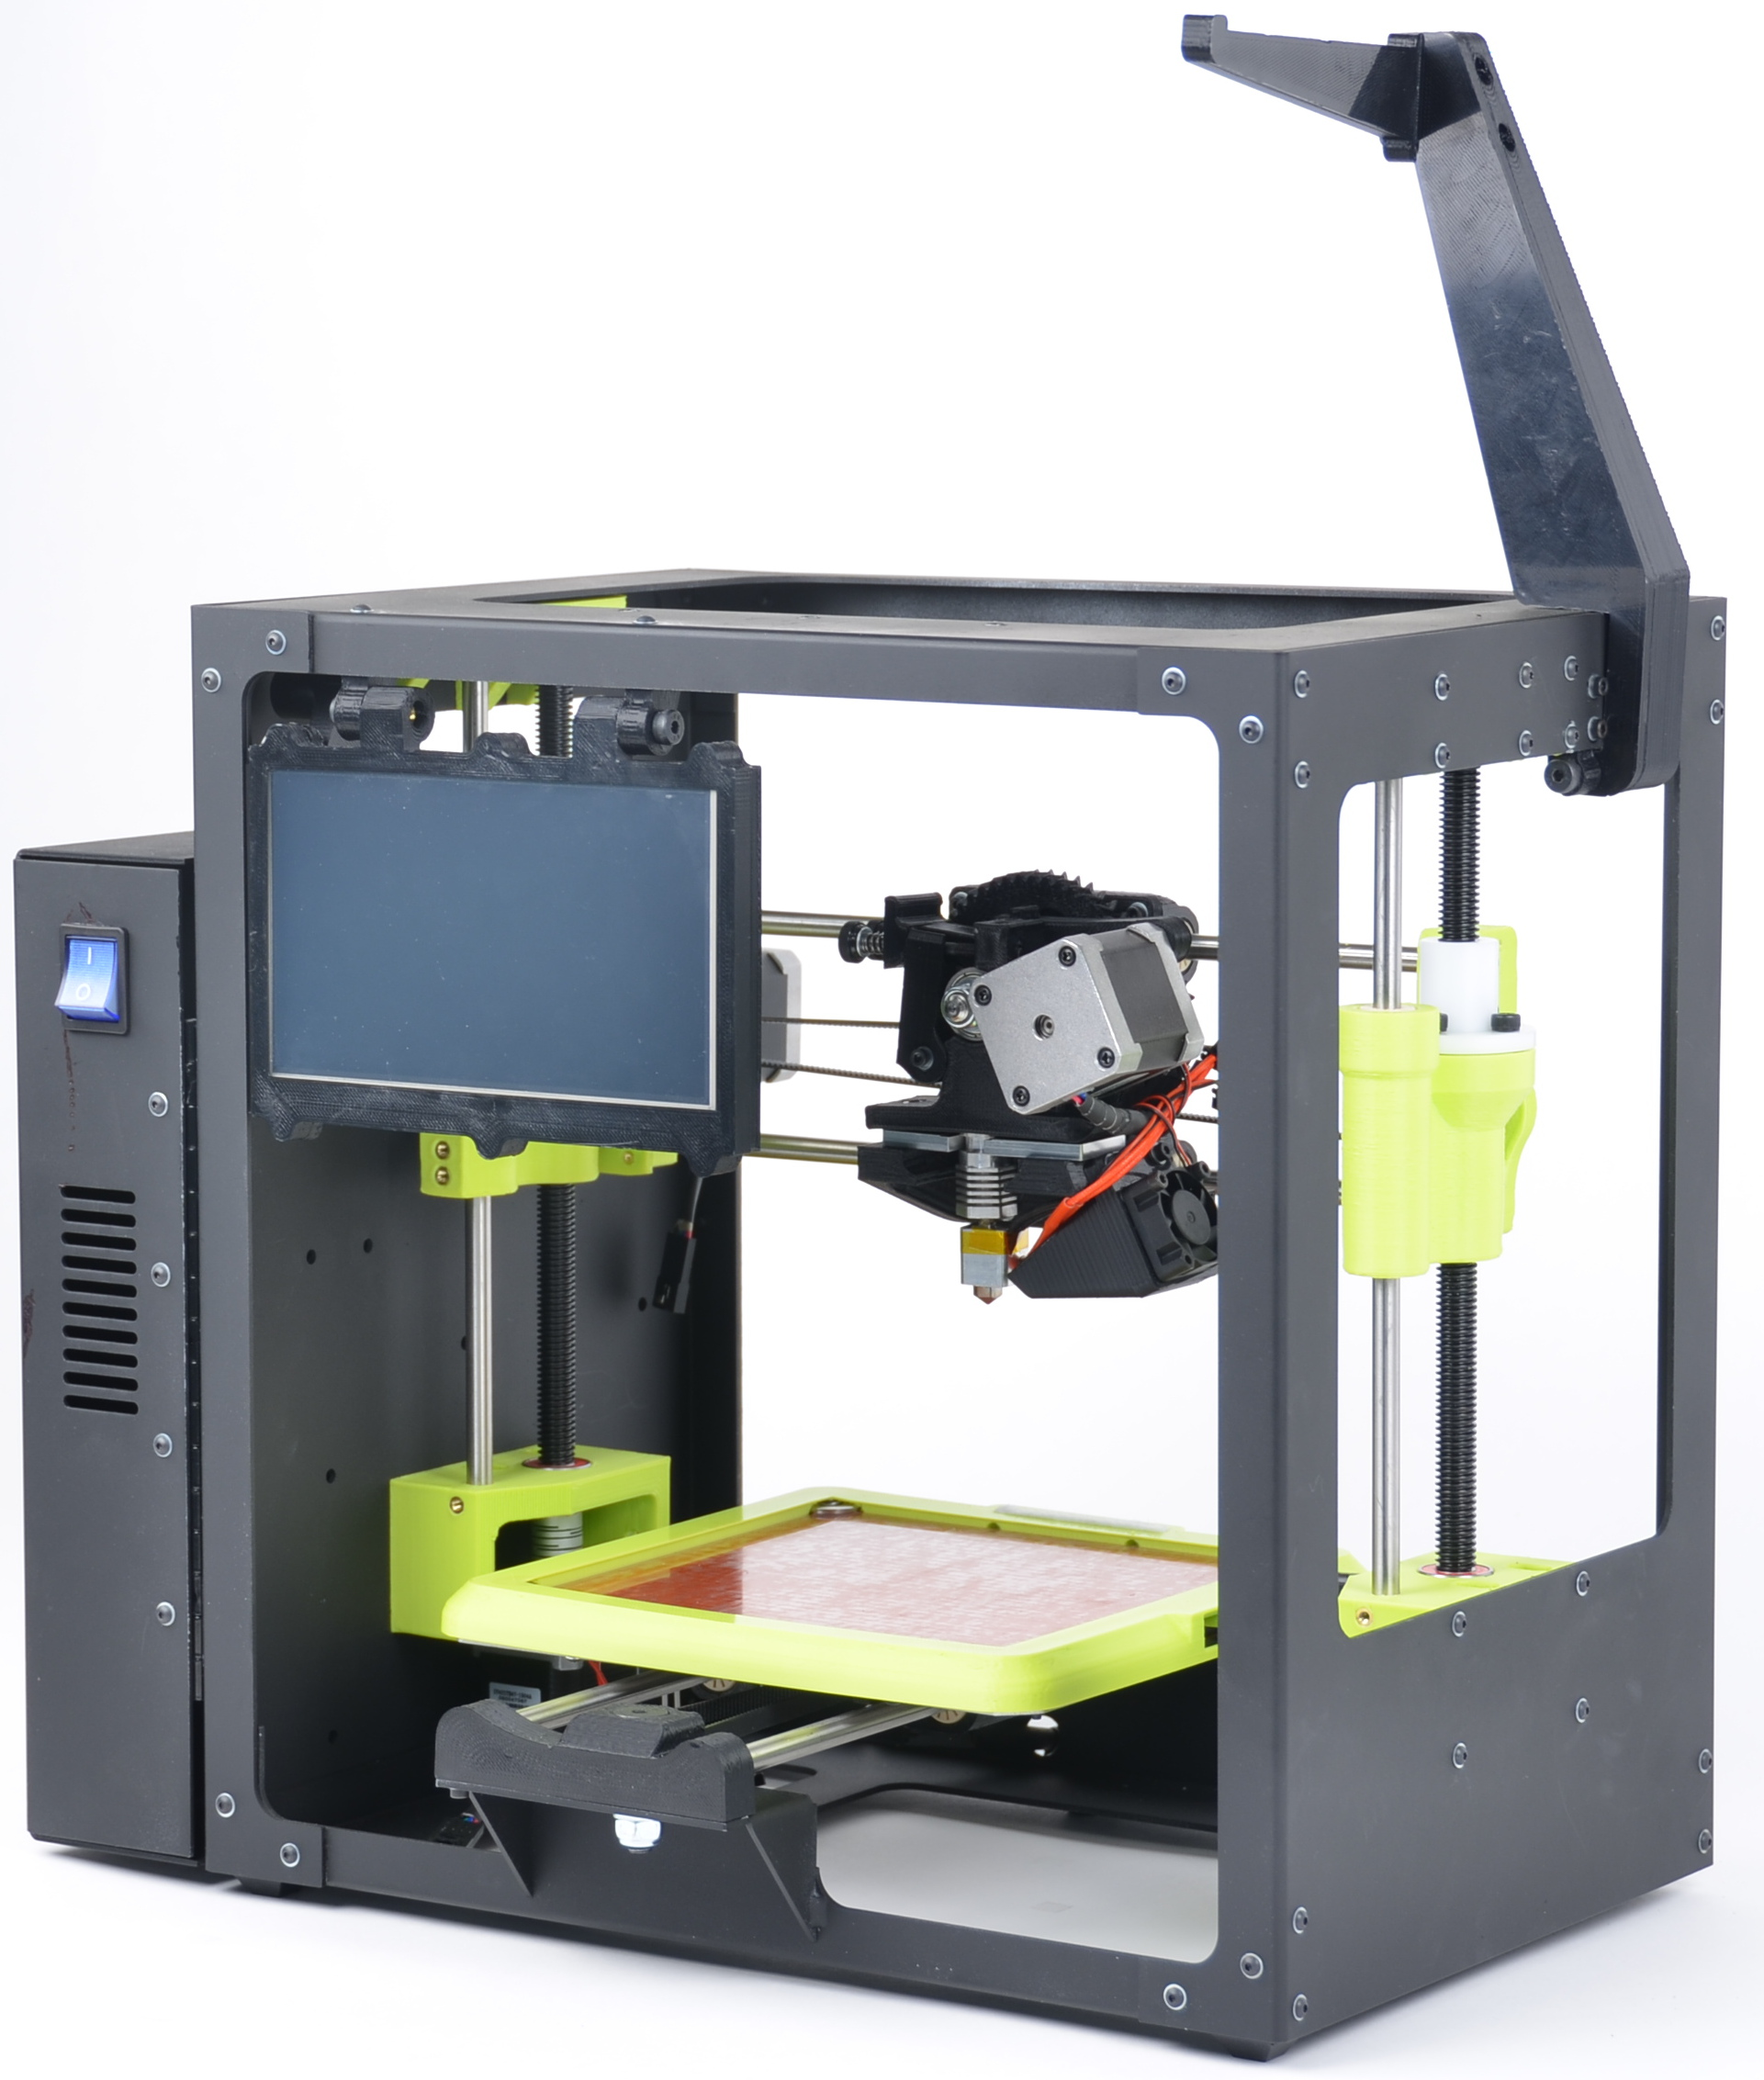
\includegraphics[keepaspectratio=true,angle=0,height=1.0\textheight,width=1.0\textwidth]{begonia/begonia-blackgreen.jpg}
\caption{Begonia Black Green Color Scheme Photo}
\label{fig:begblackgreen}
\end{figure}


\section{Schedule}
The schedule is updated weekly. It is in Libre Office spreadsheet format. The
latest version is available here:

\url{http://devel.lulzbot.com/mini/program_management/}

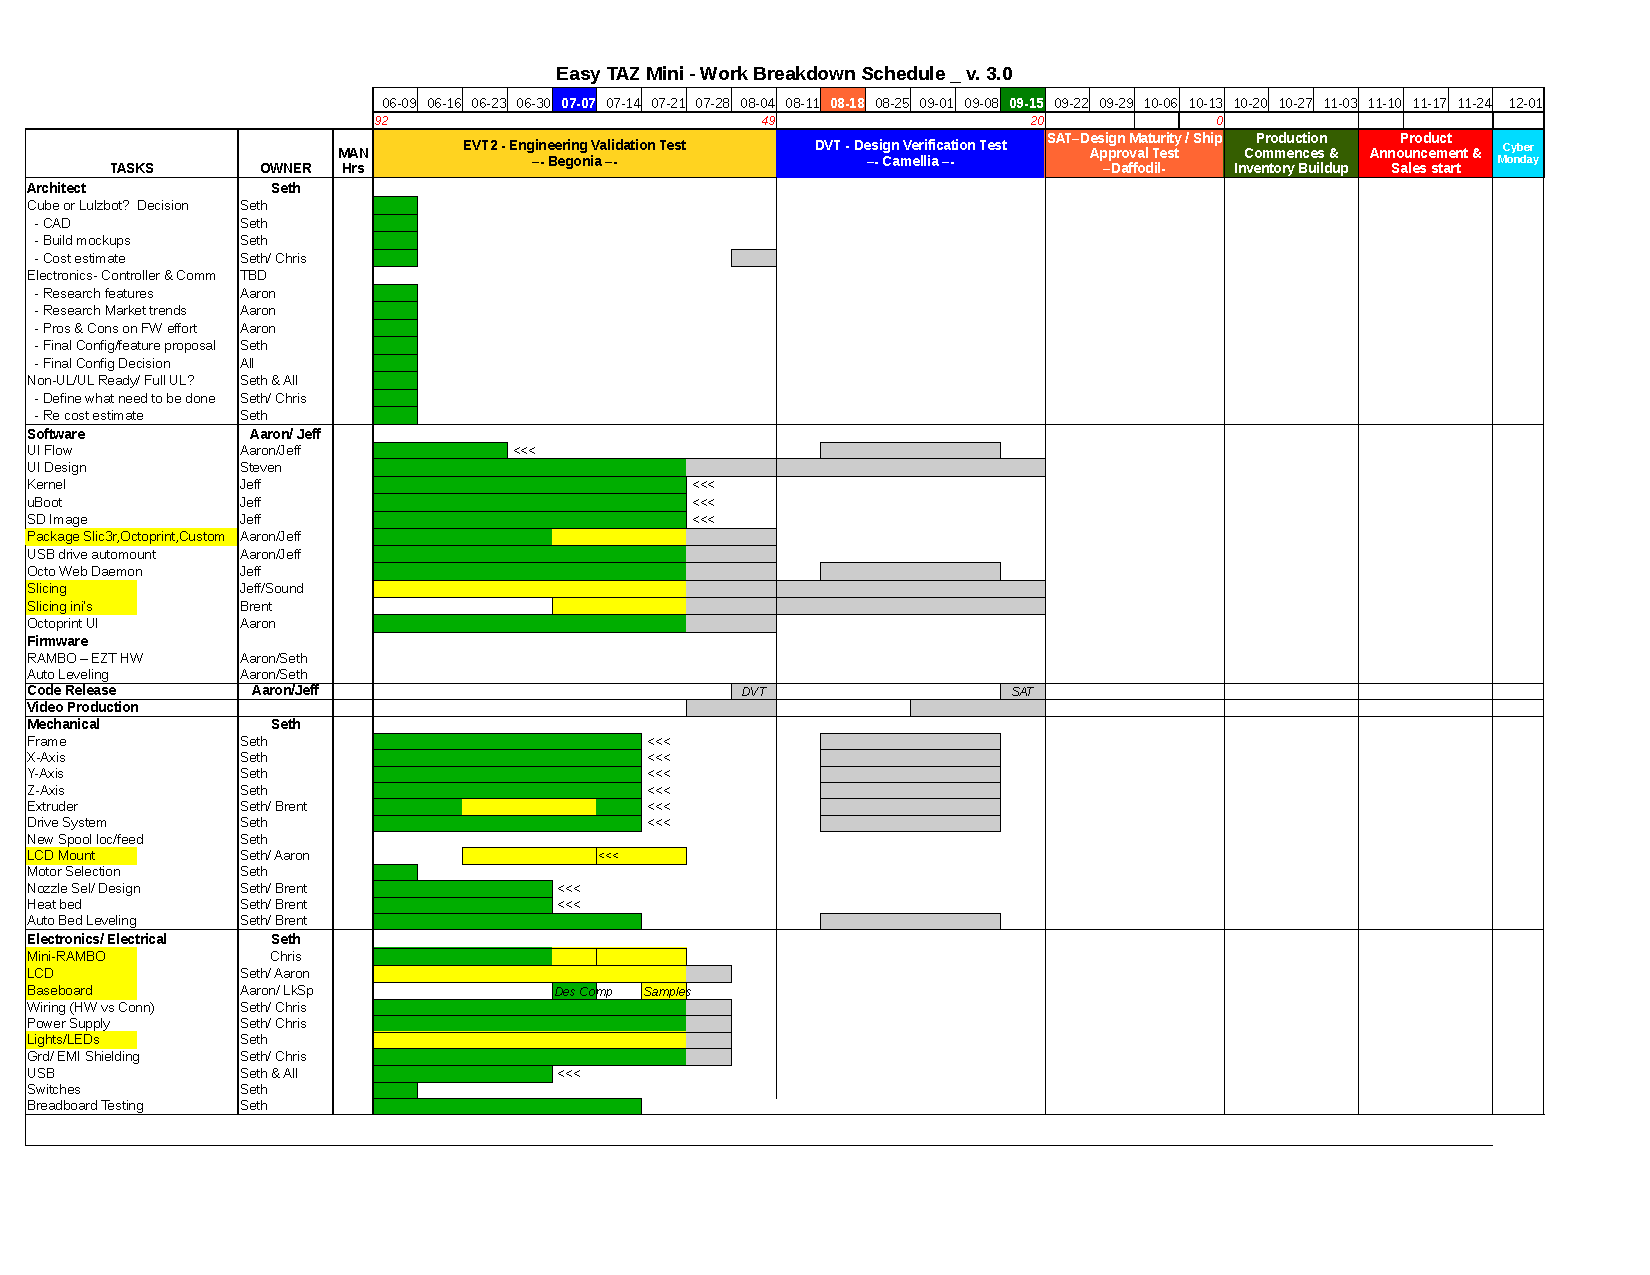
\includepdf[addtolist={1,figure,{Work Breakdown Schedule},wbs},pages=-,landscape=true,reflect=false,turn=true,fitpaper=true,keepaspectratio=true]{pm/wbs30.pdf}

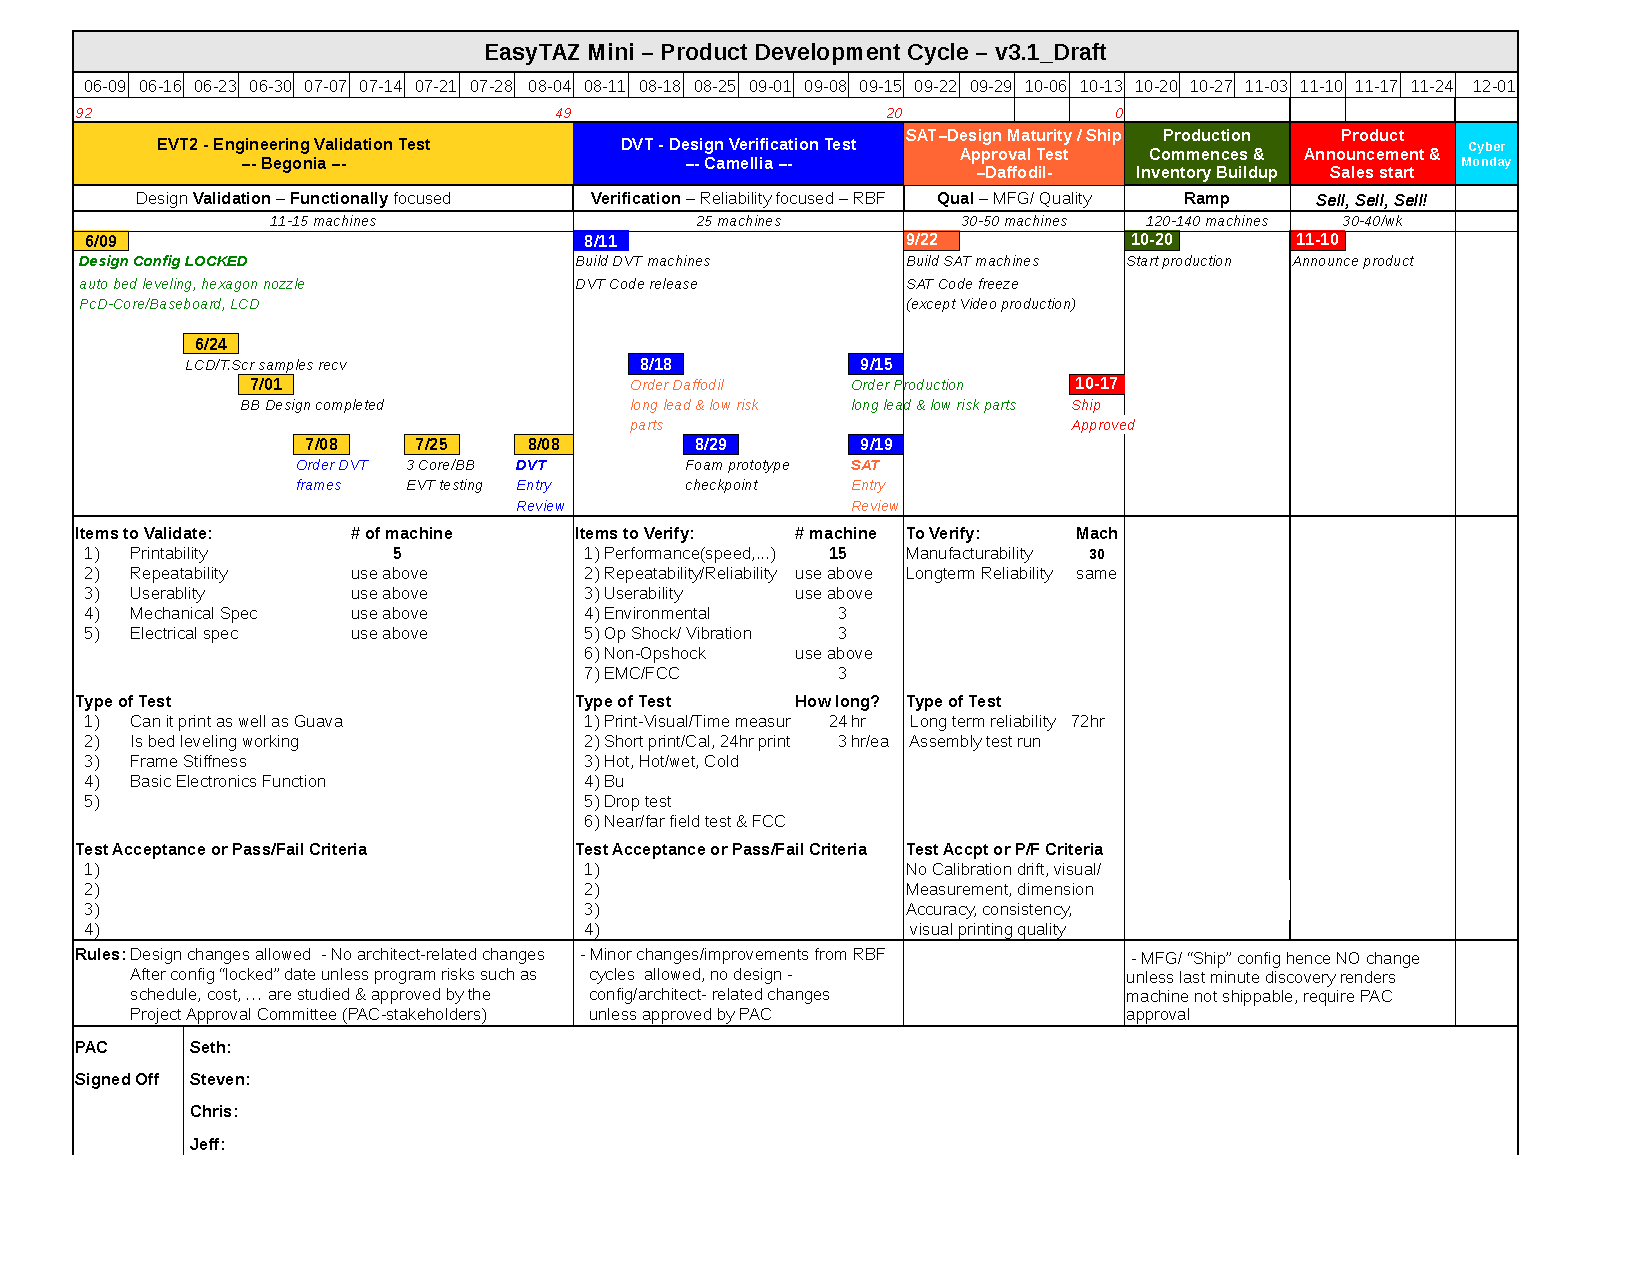
\includepdf[addtolist={1,figure,{Phase Gate Schedule},pgs},pages=-,landscape=true,reflect=false,turn=true,fitpaper=true,keepaspectratio=true]{pm/phase-gate-schedule31.pdf}


